\chapter{On computing digraph kernels}
\label{sec:17}

\abstract*{}

\abstract{}

\section{What is a graph kernel ?}
\label{sec:17.1}

We call \emph{choice} in a graph, respectively a digraph, a subset of its vertices, resp. of its nodes or actions. A choice $Y$ is called \emph{internally stable} or \emph{independent} when there exist no links --(edges) or relations (arcs)-- between its members. Furthermore, a choice $Y$ is called \emph{externally stable} when for each vertex, node or action $x$ not in $Y$, there exists at least a member $y$ of $Y$ such that $x$ is linked or related to $y$. Now, an internally \emph{and} externally stable choice is called a \emph{kernel}.  

A first trivial example is immediately given by the maximal independent vertices sets (MISs) of the $n$-cycle graph. Indeed, each MIS in the $n$-cycle graph is by definition independent, i.e. internally stable, and each non selected vertex in the $n$-cycle graph is in relation with either one or even two members of the MIS.

In all graph or symmetric digraph, the \emph{maximality condition} imposed on the internal stability is equivalent to the external stability condition. Indeed, if there would exist a vertex or node not related to any of the elements of a choice, then we may safely add this vertex or node to the given choice without violating its internal stability. All kernels must hence be maximal independent choices. In fact, in a topological sense, they correspond to maximal \emph{holes} in the given graph.

We may illustrate this coincidence between MISs and kernels in graphs
and symmetric digraphs with the following random 3-regular graph
instance.
\begin{lstlisting}
>>> from graphs import RandomRegularGraph
>>> g = RandomRegularGraph(order=12,\
...                        degree=3,seed=100)
>>> g.exportGraphViz('random3RegularGraph')
  *---- exporting a dot file for GraphViz tools --*
   Exporting to random3RegularGraph.dot
   fdp -Tpng random3RegularGraph.dot\
                   -o random3RegularGraph.png
\end{lstlisting}
\begin{figure}[h]
\sidecaption
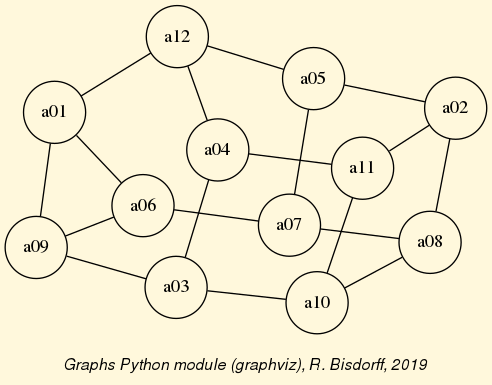
\includegraphics[width=7cm]{Figures/random3RegularGraph.png}
\caption{A random 3-regular graph instance}
\label{fig:17.1}       % Give a unique label
\end{figure}

A random MIS in this graph may be computed for instance by using the \texttt{MISModel} class.

\begin{lstlisting}
>>> from graphs import MISModel
>>> mg = MISModel(g)
  Iteration:  1
    Running a Gibbs Sampler for 660 step !
    {'a06', 'a02', 'a12', 'a10'}  is maximal !
>>> mg.exportGraphViz('random3RegularGraph_mis')
  *---- exporting a dot file for GraphViz tools ---*
   Exporting to random3RegularGraph-mis.dot
   fdp -Tpng random3RegularGraph-mis.dot\
                -o random3RegularGraph-mis.png
\end{lstlisting}
\begin{figure}[h]
\sidecaption
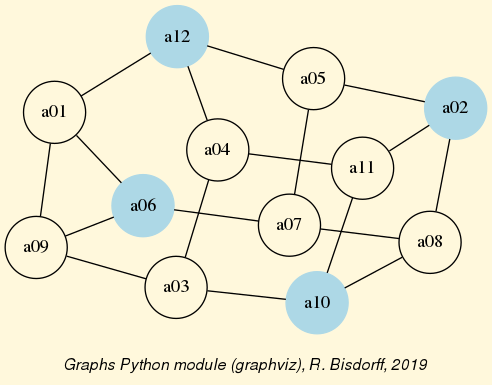
\includegraphics[width=7cm]{Figures/random3RegularGraph-mis.png}
\caption{A random MIS colored in the random 3-regular graph}
\label{fig:17.2}       % Give a unique label
\end{figure}

It is easily verified in Fig. \ref{fig:17.2} above, that the computed MIS renders indeed a valid kernel of the given graph. The complete set of kernels of this 3-regular graph instance coincides hence with the set of its MISs. 

\begin{lstlisting}
>>> g.showMIS()
    *---  Maximal Independent Sets ---*
    ['a01', 'a02', 'a03', 'a07']
    ['a01', 'a04', 'a05', 'a08']
    ['a04', 'a05', 'a08', 'a09']
    ['a01', 'a04', 'a05', 'a10']
    ['a04', 'a05', 'a09', 'a10']
    ['a02', 'a03', 'a07', 'a12']
    ['a01', 'a03', 'a07', 'a11']
    ['a05', 'a08', 'a09', 'a11']
    ['a03', 'a07', 'a11', 'a12']
    ['a07', 'a09', 'a11', 'a12']
    ['a08', 'a09', 'a11', 'a12']
    ['a04', 'a05', 'a06', 'a08']
    ['a04', 'a05', 'a06', 'a10']
    ['a02', 'a04', 'a06', 'a10']
    ['a02', 'a03', 'a06', 'a12']
    ['a02', 'a06', 'a10', 'a12']
    ['a01', 'a02', 'a04', 'a07', 'a10']
    ['a02', 'a04', 'a07', 'a09', 'a10']
    ['a02', 'a07', 'a09', 'a10', 'a12']
    ['a01', 'a03', 'a05', 'a08', 'a11']
    ['a03', 'a05', 'a06', 'a08', 'a11']
    ['a03', 'a06', 'a08', 'a11', 'a12']
    number of solutions:  22
    cardinality distribution
    card.:  [0, 1, 2, 3, 4, 5, 6, 7, 8, 9, 10, 11, 12]
    freq.:  [0, 0, 0, 0, 16, 6, 0, 0, 0, 0, 0, 0, 0]
    execution time: 0.00045 sec.
    Results in self.misset
>>> g.misset
    [frozenset({'a02', 'a01', 'a07', 'a03'}),
     frozenset({'a04', 'a01', 'a08', 'a05'}),
     frozenset({'a09', 'a04', 'a08', 'a05'}),
     ...
     ...
     frozenset({'a06', 'a02', 'a12', 'a10'}),
     frozenset({'a06', 'a11', 'a08', 'a03', 'a05'}),
     frozenset({'a03', 'a06', 'a11', 'a12', 'a08'})]
\end{lstlisting}

All graphs and symmetric digraphs admit MISs, hence also kernels. In the context of digraphs, i.e. \emph{oriented} graphs, the kernel concept gets much richer and separates from the symmetric MIS concept.  

\section{Initial and terminal kernels}
\label{sec:17.2}

In an oriented graph context, the internal stability condition of the kernel concept remains untouched; however, the external stability condition gets indeed split up by the orientation into two lateral cases:
\begin{enumerate}
\item A \emph{dominant} stability condition, where each non selected node is dominated by at least one member of the kernel;
\item An \emph{absorbent} stability condition, where each non selected node is absorbed by at least one member of the kernel.
\end{enumerate}
A both internally \textbf{and} dominant, resp. absorbent stable choice is called a dominant or \emph{initial}, resp. an absorbent or \emph{terminal} kernel. From a topological perspective, the initial kernel concept looks from the outside of the digraph into its interior, whereas the terminal kernel looks from the interior of a digraph toward its outside. From an algebraic perspective, the initial kernel is a prefix operand, and the terminal kernel is a postfix operand in the \Berge kernel equation systems (see Section \ref{17.6}).

Furthermore, as the kernel concept involves conjointly a positive logical refutation (the internal stability) and a positive logical affirmation (the external stability), it appeared rather quickly necessary in our operational developments to adopt a bipolar characteristic $[-1.0,1.0]$ valuation domain, modelling logical negation by a change of numerical sign and including explicitly a third median logical value ($0.0$) expressing logical \emph{indeterminateness} (neither positive, nor negative, see [BIS-2000] and [BIS-2004a]).

In such a  bipolar-valued context, we call \emph{prekernel} a choice which is \emph{externally stable} and for which the internal stability condition is \emph{valid or indeterminate}. We say that the independence condition is in this case only \emph{weakly} validated. Notice that all kernels are hence prekernels, but not vice-versa.

In graphs or symmetric digraphs, where there is essentially no apparent \emph{laterality}, all prekernels are initial and terminal at the same time. A universal example is given by the \emph{complete} digraph.

\begin{lstlisting}
>>> from digraphs import CompleteDigraph
>>> u = CompleteDigraph(order=5)
>>> u
  *------- Digraph instance description ------*
    Instance class   : CompleteDigraph
    Instance name    : complete
    Digraph Order      : 5
    Digraph Size       : 20
    Valuation domain : [-1.00 ; 1.00]
    ---------------------------------
>>> u.showPreKernels()
  *--- Computing preKernels ---*
   Dominant kernels :
   ['1'] ind. : 1.0; dom. : 1.0; abs. : 1.0
   ['2'] ind. : 1.0; dom. : 1.0; abs. : 1.0
   ['3'] ind. : 1.0; dom. : 1.0; abs. : 1.0
   ['4'] ind. : 1.0; dom. : 1.0; abs. : 1.0
   ['5'] ind. : 1.0; dom. : 1.0; abs. : 1.0
    Absorbent kernels :
   ['1'] ind. : 1.0; dom. : 1.0; abs. : 1.0
   ['2'] ind. : 1.0; dom. : 1.0; abs. : 1.0
   ['3'] ind. : 1.0; dom. : 1.0; abs. : 1.0
   ['4'] ind. : 1.0; dom. : 1.0; abs. : 1.0
   ['5'] ind. : 1.0; dom. : 1.0; abs. : 1.0
  *----- statistics -----
    graph name:  complete
    number of solutions
    dominant kernels :  5
    absorbent kernels:  5
    cardinality frequency distributions
    cardinality     :  [0, 1, 2, 3, 4, 5]
    dominant kernel :  [0, 5, 0, 0, 0, 0]
    absorbent kernel:  [0, 5, 0, 0, 0, 0]
    Execution time  : 0.00004 sec.
    Results in sets: dompreKernels
    and abspreKernels.
\end{lstlisting}
In a complete digraph, each single node is indeed both an initial and a terminal prekernel candidate and there is no definite begin or end of the digraph to be detected. Laterality is here entirely relative to a specific singleton chosen as reference point of view.

The same absence of laterality is apparent in two other universal digraph models, the \emph{empty} and the \emph{indeterminate} digraph. 
\begin{lstlisting}
>>> from digraphs import EmptyDigraph
>>> ed = EmptyDigraph(order=5)
>>> ed.showPreKernels()
  *--- Computing preKernels ---*
   Dominant kernel :
    ['1', '2', '3', '4', '5']
       independence :  1.0 
       dominance    :  1.0
       absorbency   :  1.0
   Absorbent kernel :
    ['1', '2', '3', '4', '5']
       independence :  1.0 
       dominance    :  1.0
       absorbency   :  1.0
\end{lstlisting}
In the empty digraph, the whole set of nodes gives indeed at the same time the unique initial and terminal prekernel. Similarly, for the indeterminate digraph.
\begin{lstlisting}
>>> from digraphs import IndeterminateDigraph
>>> id = IndeterminateDigraph(order=5)
>>> id.showPreKernels()
  *--- Computing preKernels ---*
    Dominant prekernel :
    ['1', '2', '3', '4', '5']
       independence :  0.0
       dominance    :  1.0
       absorbency   :  1.0
    Absorbent prekernel :
    ['1', '2', '3', '4', '5']
       independence :  0.0
       dominance    :  1.0
       absorbency   :  1.0
\end{lstlisting}

Both these results make sense, as in a completely empty or indeterminate digraph, there is no \emph{interior} of the digraph defined, only a \emph{border} which is hence at the same time an initial and terminal prekernel.  Notice however, that in the latter indeterminate case, the complete set of nodes verifies only weakly the internal stability condition (see above).

Other common digraph models, although being clearly oriented, may show nevertheless no apparent laterality, like \emph{odd chordless circuits}, i.e. holes surrounded by an oriented cycle -a circuit- of odd length. They do not admit in fact any initial or terminal prekernel.
\begin{lstlisting}
>>> from digraphs import CirculantDigraph
>>> c5 = CirculantDigraph(order=5,circulants=[1])
>>> c5.showPreKernels()
  *----- statistics -----
   digraph name:  c5
   number of solutions
    dominant prekernels :  0
    absorbent prekernels:  0
\end{lstlisting}

Chordless circuits of \emph{even} length $2 \times k$, with $k > 1$, contain however two isomorphic prekernels of cardinality $k$ which qualify conjointly as initial and terminal candidates.
\begin{lstlisting}
>>> c6 = CirculantDigraph(order=6,circulants=[1])
>>> c6.showPreKernels()
  *--- Computing preKernels ---*
    Dominant preKernels :
    ['1', '3', '5'] ind. : 1.0, dom. : 1.0, abs. : 1.0
    ['2', '4', '6'] ind. : 1.0, dom. : 1.0, abs. : 1.0
    Absorbent preKernels :
    ['1', '3', '5'] ind. : 1.0, dom. : 1.0, abs. : 1.0
    ['2', '4', '6'] ind. : 1.0, dom. : 1.0, abs. : 1.0
\end{lstlisting}
Chordless circuits of even length may thus be indifferently oriented along two opposite directions. Notice by the way that the duals of all chordless circuits of odd or even length, i.e. \emph{filled} circuits also called \emph{anti-holes} (see Fig. \ref{fig:17.3}), never contain any potential prekernel candidates.
\begin{lstlisting}
>>> dc6 = -c6   # dc6 = DualDigraph(c6)
>>> dc6.showPreKernels()
  *----- statistics -----
    graph name:  dual_c6
    number of solutions
     dominant prekernels :  0
     absorbent prekernels:  0
>>> dc6.exportGraphViz(fileName='dualChordlessCircuit')
  *---- exporting a dot file for GraphViz tools ----*
    Exporting to dualChordlessCircuit.dot
    circo -Tpng dualChordlessCircuit.dot\
               -o dualChordlessCircuit.png
\end{lstlisting}
\begin{figure}[h]
\sidecaption
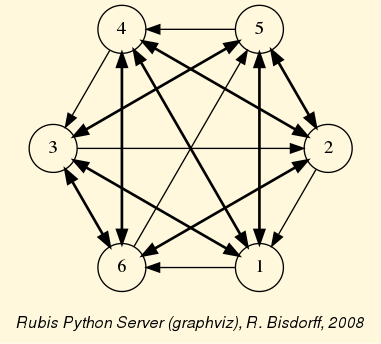
\includegraphics[width=7cm]{Figures/dualChordlessCircuit.png}
\caption{The dual of the chordless 6-circuit}
\label{fig:17.3}       % Give a unique label
\end{figure}

We call \emph{weak}, a chordless circuit with indeterminate inner part.

The \texttt{CirculantDigraph} class provides a parameter for constructing such weak chordless circuits. 
\begin{lstlisting}
>>> c6 = CirculantDigraph(order=6, circulants=[1],\
...                       IndeterminateInnerPart=True)
\end{lstlisting}
It is worth noticing that the dual version (Footnote[14]) of a weak circuit corresponds to its \emph{converse} version, i.e. $-c6$ = $\sim c6$ (see Fig. \ref{fig:17.4}).
\begin{lstlisting}
>>> (-c6).exportGraphViz()
  *---- exporting a dot file for GraphViz tools ---------*
   Exporting to dual_c6.dot
   circo -Tpng dual_c6.dot -o dual_c6.png
>>> (~c6).exportGraphViz()
  *---- exporting a dot file for GraphViz tools ---------*
   Exporting to converse_c6.dot
   circo -Tpng converse_c6.dot -o converse_c6.png 
\end{lstlisting}
\begin{figure}[h]
%\sidecaption
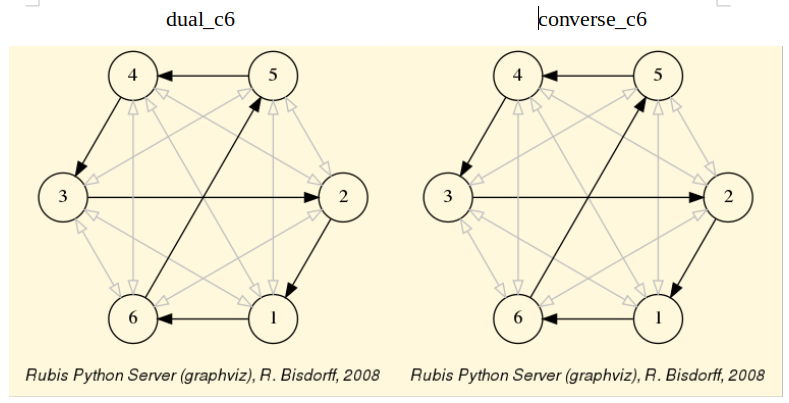
\includegraphics[width=10cm]{Figures/weakChordlessCircuit.png}
\caption{Dual and converse of the weak 6-circuit}
\label{fig:17.4}       % Give a unique label
\end{figure}

It is worthwhile noticing that weak chordless circuits of length $n$ are in fact part of the class of digraphs that are invariant under the \emph{codual} transform, $cn = - (\sim cn) = \sim (-cn )$ Footnote [13]. In the case, now, of an odd weak chordless circuit, neither the weak chordless circuit, nor its dual, converse, or codual versions will admit any initial or terminal prekernels. 

\section{Kernels in lateralized digraphs}
\label{sec:17.3}

Humans do live in an apparent physical space of plain transitive lateral orientation, fully empowered in finite geometrical 3D models with linear orders, where first, resp. last ranked, nodes deliver unique initial, resp. terminal, kernels. Similarly, in finite preorders, the first, resp. last, equivalence classes deliver the unique initial, resp. unique terminal, kernels. More generally, in finite partial orders, i.e. asymmetric and transitive digraphs, topological sort algorithms will easily reveal on the first, resp. last, level all unique initial, resp. terminal, kernels.

In genuine random digraphs, however, we may need to check for each of its MISs, whether one, both, or none of the lateralized external stability conditions may be satisfied. Consider, for instance, the following random digraph instance of order 7 and generated with an arc probability of $30\%$. 
\begin{lstlisting}
>>> from randomDigraphs import RandomDigraph
>>> rd = RandomDigraph(order=7,arcProbability=0.3,seed=5)
>>> rd.exportGraphViz('randomLaterality')
  *---- exporting a dot file for GraphViz tools ---------*
   Exporting to randomLaterality.dot
   dot -Grankdir=BT -Tpng randomLaterality.dot\
                    -o randomLaterality.png
\end{lstlisting}
\begin{figure}[h]
\sidecaption
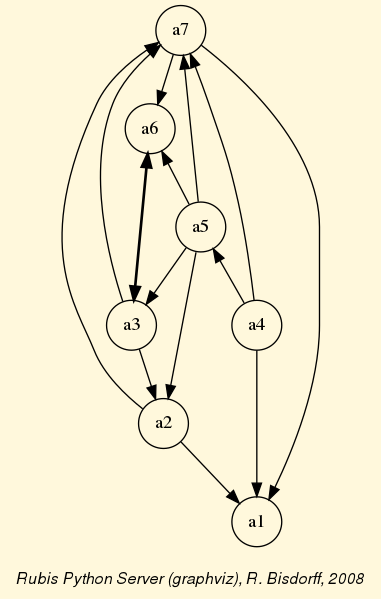
\includegraphics[width=5cm]{Figures/randomLaterality.png}
\caption{A random digraph instance of order 7 and arc probability 0.3. The digraph instance is neither asymmetric (a3 $\Leftrightarrow$ a6) nor symmetric (a2 $\rightarrow$ a1, a1 $\not\rightarrow$ a2) and, the digraph is not transitive (a5 $\rightarrow$ a2 $\rightarrow$ a1, but a5 $\not\rightarrow$ a1).} 
\label{fig:17.5}       % Give a unique label
\end{figure}
The random digraph shown in Fig. \ref{fig:17.5} has no apparent special properties, except from being connected (see Line 3 below).
\begin{lstlisting}
>>> rd.showComponents()
  *--- Connected Components ---*
  1: ['a1', 'a2', 'a3', 'a4', 'a5', 'a6', 'a7']
>>> rd.computeSymmetryDegree(Comments=True,InPercents=True)
  Symmetry degree (%) of digraph <randomDigraph>:
   arcs x>y: 14, symmetric: 1, asymmetric: 13
   symmetric/arcs =  7.1
>>> rd.computeChordlessCircuits()
  []  # no chordless circuits detected
>>> rd.computeTransitivityDegree(Comments=True,InPercents=True)
  Transitivity degree (%) of graph <randomDigraph>:
   triples x>y>z: 23, closed: 11, open: 12
   closed/triples =  47.8
\end{lstlisting}
There are no chordless circuits (see Line 9 above) and more than half of the required transitive closure is missing (see Line 12 above).

Now, we know that its potential prekernels must be among its set of maximal independent choices. 

\begin{lstlisting}
>>> rd.showMIS()
  *---  Maximal independent choices ---*
    ['a2', 'a4', 'a6']
    ['a6', 'a1']
    ['a5', 'a1']
    ['a3', 'a1']
    ['a4', 'a3']
    ['a7']
>>> rd.showPreKernels()
  *--- Computing preKernels ---*
   Dominant preKernels :
    ['a2', 'a4', 'a6']
       independence :  1.0
       dominance    :  1.0
       absorbency   :  -1.0
       covering     :  0.500
    ['a4', 'a3']
       independence :  1.0
       dominance    :  1.0
       absorbency   :  -1.0
       covering     :  0.600
   Absorbent preKernels :
    ['a3', 'a1']
       independence :  1.0
       dominance    :  -1.0
       absorbency   :  1.0
       covering     :  0.500
    ['a6', 'a1']
       independence :  1.0
       dominance    :  -1.0
       absorbency   :  1.0
       covering     :  0.600
\end{lstlisting}
     
Among the six MISs contained in this random digraph (see above Lines 3-8) we discover two initial and two terminal kernels (Lines 12-34). Notice by the way the covering values (between $0.0$ and $1.0$) shown by the \texttt{showPreKernels()} method (Lines 17, 22, 28 and 33). The higher this value, the more the corresponding prekernel candidate makes apparent the digraph's laterality. We may hence redraw the same digraph in Fig. \ref{fig:17.6} by looking into its interior via the best covering initial prekernel candidate: the dominant choice \{a3','4a'\} (coloured in yellow), and looking out of it via the best covered terminal prekernel candidate: the absorbent choice \{'a1','a6'\} (coloured in blue).

\begin{lstlisting}
>>> rd.exportGraphViz(fileName='orientedLaterality',\
...                   bestChoice=set(['a3', 'a4']),\
...                   worstChoice=set(['a1', 'a6']))
  *---- exporting a dot file for GraphViz tools ----*
   Exporting to orientedLaterality.dot
   dot -Grankdir=BT -Tpng orientedLaterality.dot\
                    -o orientedLaterality.png
\end{lstlisting}

\begin{figure}[h]
\sidecaption
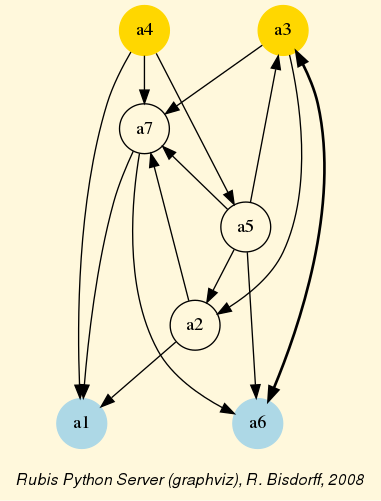
\includegraphics[width=7cm]{Figures/orientedLaterality.png}
\caption{A random digraph oriented by best covering initial and
   best covered terminal kernel}
\label{fig:17.6}       % Give a unique label
\end{figure}

In Algorithmic Decision Theory, initial and terminal prekernels may provide convincing best, resp. last, choice recommendations.


\section{Computing first and last choice recommendations}
\label{sec:17.4}

To illustrate this idea, let us finally compute first and last choice recommendations in the following random bipolar-valued outranking digraph.
\begin{lstlisting}
>>> from outrankingDigraphs import\
...                RandomBipolarOutrankingDigraph
>>> g = RandomBipolarOutrankingDigraph(seed=5)
>>> g
  *------- Object instance description ------*
   Instance class   : RandomBipolarOutrankingDigraph
   Instance name    : randomOutranking
   Actions          : 7
   Criteria         : 7
   Size             : 26
   Determinateness  : 34.275
   Valuation domain : {'min': -100.0, 'med': 0.0, 'max': 100.0}
>>> g.showHTMLPerformanceTableau()
\end{lstlisting}
\begin{figure}[h]
%\sidecaption
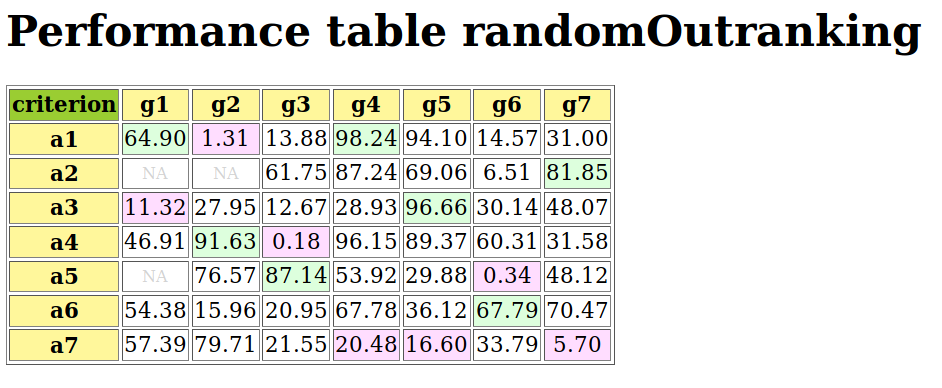
\includegraphics[width=10cm]{Figures/randomOutranking.png}
\caption{The performance tableau of a random outranking digraph instance}
\label{fig:17.7}       % Give a unique label
\end{figure}

The underlying random performance tableau shown in Fig. \ref{fig:17.7} reveals the performance grading of 7 potential decision actions with respect to 7 decision criteria supporting each an increasing performance scale from $0.0$ to $100.0$. Notice the missing performance data concerning decision actions 'a2' and 'a5'. The resulting \emph{strict} outranking - i.e. a weighted majority supported --\emph{better than without considerable counter-performance}-- digraph is shown in Fig. \ref{fig:17.8}.
\begin{lstlisting}
>>> gcd = ~(-g)  # Codual: the converse of the negation
>>> gcd.exportGraphViz(fileName='tutOutRanking')
  *---- exporting a dot file for GraphViz tools ----*
   Exporting to tutOutranking.dot
   dot -Grankdir=BT -Tpng tutOutranking.dot\
                    -o tutOutranking.png
\end{lstlisting}
\begin{figure}[h]
\sidecaption
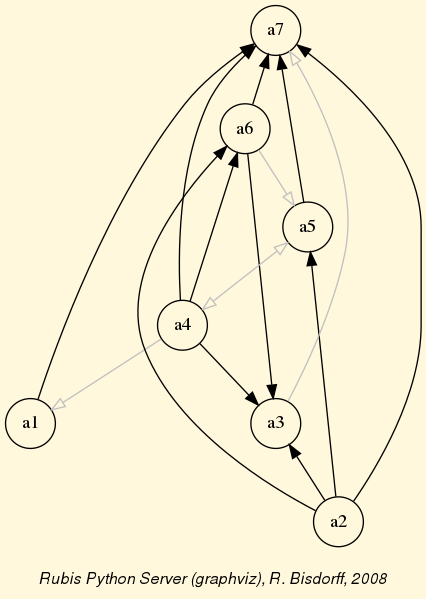
\includegraphics[width=6cm]{Figures/tutOutranking.png}
\caption{A random strict outranking digraph instance. All decision actions appear strictly better performing than action a7. We call it a \Condorcet loser and it is an evident terminal prekernel candidate. On the other side, three actions: a1, a2 and a4 are not dominated. They give together an initial prekernel candidate.}
\label{fig:17.8}       % Give a unique label
\end{figure}
\begin{lstlisting}
>>> gcd.showPreKernels()
  *--- Computing preKernels ---*
   Dominant preKernels :
    ['a1', 'a2', 'a4']
       independence :  0.00
       dominance    :  6.98
       absorbency   :  -48.84
       covering     :  0.667
   Absorbent preKernels :
    ['a3', 'a7']
       independence :  0.00
       dominance    :  -74.42
       absorbency   :  16.28
       covered      :  0.800
\end{lstlisting}

With such unique disjoint initial and terminal prekernels (see Line 4 and 10), the given digraph instance is hence clearly lateralized. Indeed, these initial and terminal prekernels of the codual outranking digraph reveal best, resp. worst, choice recommendations one may formulate on the basis of a given outranking digraph instance.
\begin{lstlisting}
>>> g.showBestChoiceRecommendation()
  Rubis best choice recommendation(s) (BCR)
   (in decreasing order of determinateness)   
   Credibility domain: [-100.00,100.00]
   === >> potential best choice(s)
    * choice              : ['a1', 'a2', 'a4']
      independence        : 0.00
      dominance           : 6.98
      absorbency          : -48.84
      covering (%)        : 66.67
      determinateness (%) : 57.97
      - most credible action(s) =
                      {'a4': 20.93,'a2': 20.93}
   === >> potential worst choice(s) 
    * choice              : ['a3', 'a7']
      independence        : 0.00
      dominance           : -74.42
      absorbency          : 16.28
      covered (%)         : 80.00
      determinateness (%) : 64.62
      - most credible action(s) = { 'a7': 48.84, }
\end{lstlisting}

Notice that solving the valued \Berge kernel equations provides furthermore a positive characterization of the most credible decision actions in each respective choice recommendation (see Lines 14 and 23 above). Actions 'a2' and 'a4' are equivalent candidates for a unique best choice, and action 'a7' is clearly confirmed as the worst choice.

In Fig. \ref{fig:17.8}, we orient the drawing of the strict outranking digraph instance with the help of these best and worst choice recommendations. 
\begin{lstlisting}
>>> gcd.exportGraphViz(fileName='bestWorstOrientation',\
...                    bestChoice=['a2','a4'],\
...                    worstChoice=['a7'])
  *---- exporting a dot file for GraphViz tools -----*
   Exporting to bestWorstOrientation.dot
   dot -Grankdir=BT -Tpng bestWorstOrientation.dot\
                    -o bestWorstOrientation.png
\end{lstlisting}
\begin{figure}[h]
\sidecaption
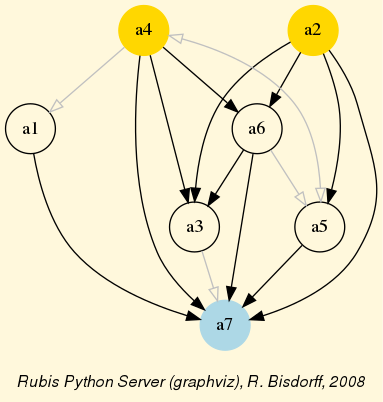
\includegraphics[width=7cm]{Figures/bestWorstOrientation.png}
\caption{The strict outranking digraph oriented by its best and worst choice recommendations. The gray arrows, like the one between actions a4 and a1, represent indeterminate preferential situations. Action a1 appears hence to be rather incomparable to all the other, except action a7.}
\label{fig:17.8}       % Give a unique label
\end{figure}

It may be interesting to compare this result with a \Copeland ranking of the underlying performance tableau (see Chapter 8 \ref{sec:8} on ranking with uncommensurable criteria).
\begin{lstlisting}
>>> g.showHTMLPerformanceHeatmap(colorLevels=5, ndigits=0,\
...             Correlations=True, rankingRule='Copeland')
\end{lstlisting}
\begin{figure}[h]
%\sidecaption
\includegraphics[width=10cm]{Figures/outRankingResult.png}
\caption{Heatmap with Copeland ranking of the performance tableau}
\label{fig:17.9}       % Give a unique label
\end{figure}

In the resulting linear ranking (see Fig. \ref{fig:17.9}), action 'a4' is set at first rank, followed by action 'a2'. This makes sense as 'a4' shows three performances in the first quintile, whereas 'a2' is only partially evaluated and shows only two such excellent performances. But 'a4' also shows a very weak performance in the first quintile. Both decision actions, hence, don't show eventually a performance profile that would make apparent a clear preference situation in favour of one or the other. In this sense, the prekernels based best choice recommendations may appear more faithful with respect to the actually definite strict outranking relation than any 'forced' linear ranking result as shown in Fig. \ref{fig:17.9}.

\section{Tractability of prekernel computation}
\label{sec:17.5}

Let us give some hints on the \emph{tractability} of prekernel computations. Detecting all prekernels in a digraph is a famously NP-hard computational problem. Checking external stability conditions for an independent choice is equivalent to checking its maximality and may be done in the linear complexity of the order of the digraph. However, checking all independent choices contained in a digraph may get hard already for tiny sparse digraphs of order $n > 20$ (see [BIS-2006b]). Indeed, the worst case is given by an empty or indeterminate digraph where the set of all potential independent choices to check is in fact the power set of the vertices.
\begin{lstlisting}
>>> e = EmptyDigraph(order=20)
>>> e.showMIS()   # by visiting all 2^20 independent choices
  *---  Maximal independent choices ---*
    [ '1', '2', '3', '4', '5', '6', '7', '8', '9','10',
     '11','12','13','14','15','16','17','18','19','20']
    number of solutions:  1
    execution time: 1.47640 sec.
>>> 2**20
  1048576
\end{lstlisting}

Now, there exist more efficient specialized algorithms for directly enumerating MISs and dominant or absorbent kernels contained in specific digraph models without visiting all independent choices (see [BIS-2006b]). \emph{Alain Hertz} provided kindly such a MISs enumeration algorithm for the \Digraph project (the \texttt{showMIS\_AH()} method). When the number of independent choices is big compared to the actual number of MISs, like in very sparse or empty digraphs, the performance difference may be dramatic (see Line 7 above and Line 15 below).
\begin{lstlisting}
>>> e.showMIS_AH()
  # by visiting only maximal independent choices
  *-----------------------------------*
  * Python implementation of Hertz's  *
  * algorithm for generating all MISs *
  * R.B. version 7(6)-25-Apr-2006     *
  *-----------------------------------*
  ===>>> Initial solution :
  [ '1','2','3','4','5','6','7','8','9','10','11',
    '12','13','14','15','16','17','18','19','20']
  *---- results ----*
  [ '1','2','3','4','5','6','7','8','9','10','11',
    '12','13','14','15','16','17','18','19','20']
  *---- statistics ----*
  MIS solutions    :  1
  execution time   : 0.00026 sec.
  iteration history:  1
\end{lstlisting}

For more or less dense strict outranking digraphs of modest order, as facing usually in Algorithmic Decision Theory applications, enumerating all independent choices remains however in most cases tractable, especially by using a very efficient Python generator (see the \texttt{independentChoices()} method below).
\begin{lstlisting}
def independentChoices(self,U):
    """
    Generator for all independent choices with associated
    dominated, absorbed and independent neighborhoods
    of digraph instance self.
    Initiate with U = self.singletons().
    Yields [(independent choice, domnb, absnb, indnb)].
    """
    if U == []:
        yield [(frozenset(),set(),set(),set(self.actions))]
    else:
        x = list(U.pop())
        for S in self.independentChoices(U):
            yield S
            if x[0] <=  S[0][3]:
                Sxgamdom = S[0][1] | x[1]
                Sxgamabs = S[0][2] | x[2]
                Sxindep = S[0][3] &  x[3]
                Sxchoice = S[0][0] | x[0]
                Sx = [(Sxchoice,Sxgamdom,Sxgamabs,Sxindep)]
                yield Sx
\end{lstlisting}

And, checking maximality of independent choices via the external stability conditions during their enumeration with the \texttt{computePreKernels()} method (see below) provides the effective advantage of computing all initial and terminal prekernels in a single loop (see Line 10 and [BIS-2006b]).
\begin{lstlisting}[caption={Computing dominant and absorbent preKernels},label=list:17.1]
def computePreKernels(self):
    """
    computing dominant and absorbent preKernels:
    Result in self.dompreKernels and self.abspreKernels
    """
    actions = set(self.actions)
    n = len(actions)
    dompreKernels = set()
    abspreKernels = set()
    for choice in self.independentChoices(self.singletons()):
        restactions = actions - choice[0][0]
        if restactions <= choice[0][1]:
            dompreKernels.add(choice[0][0])
        if restactions <= choice[0][2]:
            abspreKernels.add(choice[0][0])
    self.dompreKernels = dompreKernels
    self.abspreKernels = abspreKernels
\end{lstlisting}
 
Finally, we use our bipolar epistemic logic framework for computing the credibility that an individual node of the digraph fits with being a member of an initial or terminal prekerenel. For this purpose we make use of the \Berge kernel equation systems Footnote[x][BER-1958p].

\section{\Berge kernel equation systems}
\label{sec:117:6}

Let $G(X,R)$ be a crisp irreflexive digraph defined on a finite set $X$ of nodes and where $R$ is the corresponding $\{-1,+1\}$-valued adjacency matrix. Let $Y$ be the $\{-1,+1\}$-valued membership characteristic (row) vector of a choice in $X$.

When $Y$ satisfies the following equation system: $Y \circ R \; = \; -Y$, where for all $x$ in $X$,
\begin{equation}\label{eq:17.2}
     (Y \circ R)(x) \; = \; \max_{y \in X, x \neq y} \big ( \min(Y(x), R(x,y))\big)\;,`
\end{equation}
then $Y$ characterises an \emph{initialkernel} ([BER-1958p]).

When transposing now the membership characteristic vector $Y$ into a column vector $Y^t$, the following equation system: $R \circ Y^t \; = \; -Y^t$.
makes $Y^t$ similarly characterise a \emph{terminal kernel}.

Let us verify this result on a tiny random digraph.
\begin{lstlisting}
>>> from digraphs import RandomDigraph
>>> g = RandomDigraph(order=3,seed=1)
>>> g.showRelationTable()
  * ---- Relation Table -----
     R  | 'a1'  'a2'  'a3'	  
  ------|---------------------
   'a1' |  -1    +1    -1	 
   'a2' |  -1    -1    +1	 
   'a3' |  +1    +1    -1	 
>>> g.showPreKernels()
  *--- Computing preKernels ---*
   Dominant preKernels :
    ['a3']
     independence :  1.0
     dominance    :  1.0
     absorbency   :  -1.0
     covering     :  1.000
   Absorbent preKernels :
    ['a2']
     independence :  1.0
     dominance    :  -1.0
     absorbency   :  1.0
     covered      :  1.000
\end{lstlisting}
It is easy to verify that the characteristic vector $[-1, -1, +1]$ satisfies the initial kernel equation system; 'a3' gives an \emph{initial} kernel. Similarly, the characteristic vector $[-1, +1, -1]$ verifies indeed the terminal kernel equation system and hence 'a2' gives a \emph{terminal} kernel.

We succeeded now in generalizing \Berge's kernel equation systems to genuine bipolar-valued digraphs ([BIS-2006-1p]). The constructive proof, found by \emph{Marc Pirlot}, is based on the following \emph{fixpoint equation} that may be used for computing bipolar-valued kernel membership vectors,
\begin{equation}\label{eq:17.4}
T(Y) \; := \; -(Y \circ R) = Y\;,
\end{equation}
\emph{John von Neumann} showed indeed that, when a digraph $G(X,R)$ is acyclic with a unique initial kernel $K$ characterised by its membership characteristics vector $Y_k$, then the following double bipolar-valued fixpoint equation:
\begin{equation}\label{eq:17.5}
T^2(Y) \; := \; -\big( -(Y \circ R) \circ R) \; = \; Y\;.
\end{equation}
will admit a stable high and a stable low fixpoint solution that converge both to $Y_k$ ([SCH-1985p]).

Inspired by this crisp double fixpoint equation, we observed that for a given bipolar-valued digraph $G(X,R)$, each of its dominant or absorbent prekernels $K_i$ in $X$ determines an induced partial digraph $G(X,R/K_i)$ which is acyclyc and admits $K_i$ as unique kernel (see [BIS-2006-2p]).

Following the \emph{von Neumann} fixpoint algorithm, a similar bipolar-valued extended double fixpoint algorithm, applied to $G(X,R/K_i)$, allows us to compute hence the associated bipolar-valued kernel characteristic vectors $Y_i$ in polynomial complexity.

\noindent \textbf{Algorithm} 
\begin{itemize}
 \item [] \emph{in} : bipolar-valued digraph $G(X,R)$,
 \item [] \emph{out} : set $\{Y_1, Y_2, .. \}$ of bipolar-valued kernel membership characteristic vectors.
\end{itemize}
\begin{enumerate}
\item Enumerate all initial and terminal prekernels $K_1$, $K_2$, ... in the given bipolar-valued digraph (see Listing \ref{list:17.1});
\item For each crisp initial kernel $K_i$:
  \begin{enumerate}
  \item Construct a partially determined subgraph $G(X,R/K_i)$ supporting exactly this unique initial kernel $K_i$;
  \item Use the double fixpoint equation $T^2$ \ref{eq:17.5} with the partially determined adjacency matrix $R/K_i$ for computing a stable low and a stable high fixpoint;
   \item Determine the bipolar-valued $K_i$-membership characteristic vector $Y_i$ with an epistemic disjunction of the previous low and high fixpoints;
  \end{enumerate}
\item Repeat step (2) for each terminal kernel $K_j$ by using the double fixpoint equation $T^2$ with the transpose of the adjacency matrix $R/K_j$.
\end{enumerate}

Time for a practical illustration.
\begin{lstlisting}
>>> from outrankingDigraphs import \
           RandomBipolarOutrankingDigraph
>>> g = RandomBipolarOutrankingDigraph(seed=5)
>>> g
  *------- Object instance description ------*
   Instance class      : RandomBipolarOutrankingDigraph
   Instance name       : rel_randomperftab
   Actions             : 7
   Criteria            : 7
   Size                : 26
   Determinateness (%) : 67.14
   Valuation domain    : [-1.0;1.0]
   Attributes          : ['name', 'actions', 'criteria',
                          'evaluation', 'relation',
                          'valuationdomain', 'order',
                          'gamma', 'notGamma']
\end{lstlisting}
The random outranking digraph $g$, we consider above for illustration, models the pairwise outranking situations between seven decision alternatives evaluated on seven incommensurable performance criteria. We compute its corresponding bipolar-valued prekernels on the associated codual digraph $gcd$.
\begin{lstlisting}
>>> gcd = ~(-g) # strict outranking digraph
>>> gcd.showPreKernels()
  *--- Computing prekernels ---*
   Dominant prekernels :
    ['a1', 'a4', 'a2']
       independence :  +0.000
       dominance    :  +0.070
       absorbency   :  -0.488
       covering     :  +0.667
   Absorbent prekernels :
    ['a7', 'a3']
       independence :  +0.000
       dominance    :  -0.744
       absorbency   :  +0.163
       covered      :  +0.800
  *----- statistics -----
   graph name:  converse-dual_rel_randomperftab
   number of solutions
    dominant kernels :  1
    absorbent kernels:  1
   cardinality frequency distributions
    cardinality     :  [0, 1, 2, 3, 4, 5, 6, 7]
    dominant kernel :  [0, 0, 0, 1, 0, 0, 0, 0]
    absorbent kernel:  [0, 0, 1, 0, 0, 0, 0, 0]
   Execution time  : 0.00022 sec.
\end{lstlisting}
The codual outranking digraph, modelling a strict outranking relation, admits an initial prekernel ['a1', 'a2', 'a4'] and a terminal one ['a3', 'a7'] (see Lines 5 and 11).

We may now compute the initial prekernel restricted adjacency table with the \texttt{domkernelrestrict()} method.
\begin{lstlisting}
>>> k1Relation = gcd.domkernelrestrict(['a1','a2','a4'])
>>> gcd.showHTMLRelationTable(\
...      actionsList=['a1','a2','a4','a3','a5','a6','a7'],\
...      relation=k1Relation,\
...      tableTitle='K1 restricted adjacency table')
\end{lstlisting}
\begin{figure}[h]
\sidecaption
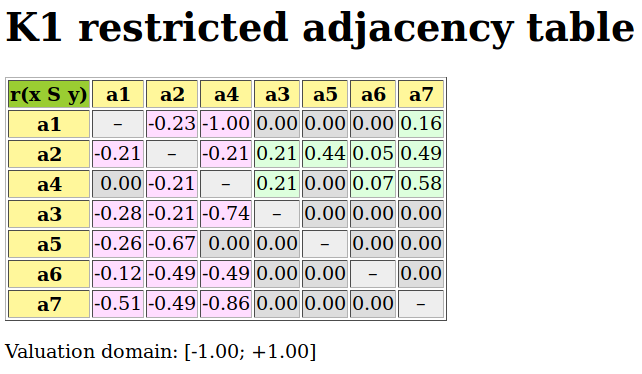
\includegraphics[width=7cm]{Figures/k1restricted.png}
\caption{Initial kernel ['a1','a2','a4'] restricted adjacency table. This initial prekernel is indeed only weakly independent: The outranking situation between 'a4' and 'a1' is indeed \emph{indeterminate}. }
\label{fig:17.10}       % Give a unique label
\end{figure}

The corresponding initial prekernel membership characteristic vector may be computed with the \texttt{computeKernelVector()} method.
\begin{lstlisting}[caption={Fixpoint iterations for initial prekernel ['a1','a2','a4']},label=list:17.2]
>>> gcd.computeKernelVector(['a1','a2','a4'],\
...                 Initial=True,Comments=True)
 --> Initial prekernel: {'a1', 'a2', 'a4'}
 initial low vector : [-1.00,-1.00,-1.00,-1.00,-1.00,-1.00,-1.00]
 initial high vector: [+1.00,+1.00,+1.00,+1.00,+1.00,+1.00,+1.00]
 1st low vector     : [ 0.00,+0.21,-0.21, 0.00,-0.44,-0.07,-0.58]
 1st high vector    : [+1.00,+1.00,+1.00,+1.00,+1.00,+1.00,+1.00]
 2nd low vector     : [ 0.00,+0.21,-0.21, 0.00,-0.44,-0.07,-0.58]
 2nd high vector    : [ 0.00,+0.21,-0.21,+0.21,-0.21,-0.05,-0.21]
 3rd low vector     : [ 0.00,+0.21,-0.21,+0.21,-0.21,-0.07,-0.21]
 3rd high vector    : [ 0.00,+0.21,-0.21,+0.21,-0.21,-0.05,-0.21]
 4th low vector     : [ 0.00,+0.21,-0.21,+0.21,-0.21,-0.07,-0.21]
 4th high vector    : [ 0.00,+0.21,-0.21,+0.21,-0.21,-0.07,-0.21]
 Iterations         : 4
 low & high fusion  : [ 0.00,+0.21,-0.21,+0.21,-0.21,-0.07,-0.21]
 Choice vector for initial prekernel: {'a1', 'a2', 'a4'}
   'a2': +0.21
   'a4': +0.21
   'a1':  0.00
   'a6': -0.07
   'a3': -0.21
   'a5': -0.21
   'a7': -0.21
\end{lstlisting}
We start in Listing \ref{list:17.2} the fixpoint computation with an empty set characterisation as first low vector and a complete set $X$ characterising high vector. After each iteration, the low vector is set to the negation of the previous high vector and the high vector is set to the negation of the previous low vector.

A unique stable prekernel characteristic vector $Y_1$ is here attained at the fourth iteration with positive members 'a2': $+0.21$ and 'a4': $+0.21$ ($60.5\%$ criteria significance majority); 'a1': $0.00$ being an ambiguous potential member. Alternatives 'a3', 'a5', 'a6' and 'a7' are all negative members, i.e. positive \emph{non members} of this outranking prekernel.

Let us now compute the restricted adjacency table for the outranked, i.e. the \emph{terminal} prekernel ['a3','a7'].
\begin{lstlisting}
>>> k2Relation = gcd.abskernelrestrict(['a3','a7'])
>>> gcd.showHTMLRelationTable(\
...   actionsList=['a3','a7','a1','a2','a4','a5','a6'],\
...   relation=k2Relation,\
...   tableTitle='K2 restricted adjacency table')
\end{lstlisting}
\begin{figure}[h]
\sidecaption
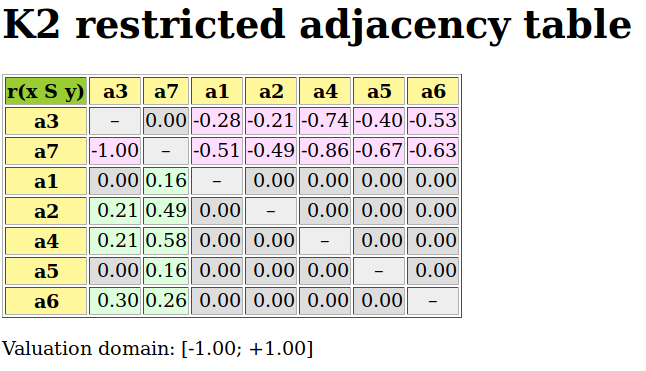
\includegraphics[width=7cm]{Figures/k2restricted.png}
\caption{Terminal prekernel ['a3','a7'] restricted adjacency table. Again, we notice that this terminal prekernel is indeed only weakly independent.}
\label{fig:17.10}       % Give a unique label
\end{figure}

The corresponding bipolar-valued characteristic vector $Y_2$ may be computed as follows.
\begin{lstlisting}
>>> gcd.computeKernelVector(['a3','a7'],Initial=False,Comments=True)
 --> Terminal prekernel: {'a3', 'a7'}
 initial low vector  : [-1.00,-1.00,-1.00,-1.00,-1.00,-1.00,-1.00]
 initial high vector : [+1.00,+1.00,+1.00,+1.00,+1.00,+1.00,+1.00]
 1st low vector      : [-0.16,-0.49, 0.00,-0.58,-0.16,-0.30,+0.49]
 1st high vector     : [+1.00,+1.00,+1.00,+1.00,+1.00,+1.00,+1.00]
 2nd low vector      : [-0.16,-0.49, 0.00,-0.58,-0.16,-0.30,+0.49]
 2nd high vector     : [-0.16,-0.49, 0.00,-0.49,-0.16,-0.26,+0.49]
 3rd low vector      : [-0.16,-0.49, 0.00,-0.49,-0.16,-0.26,+0.49]
 3rd high vector     : [-0.16,-0.49, 0.00,-0.49,-0.16,-0.26,+0.49]
 Iterations          : 3
 high & low fusion   : [-0.16,-0.49, 0.00,-0.49,-0.16,-0.26,+0.49]
 Choice vector for terminal prekernel: {'a3','a7'}
    'a7': +0.49
    'a3':  0.00
    'a1': -0.16
    'a5': -0.16
    'a6': -0.26
    'a2': -0.49
    'a4': -0.49
\end{lstlisting}

A unique stable bipolar-valued high and low fixpoint is attained at the third iteration with '7' positively confirmed (about $75\%$ criteria significance majority) as member of this terminal prekernel, whereas the membership of 'a3' in this prekernel appears indeterminate. All the remaining nodes have negative membership characteristic values and are hence positively excluded from this prekernel.

When we reconsider the graphviz drawing of this outranking digraph in Fig. \ref{fig:17.8},
\begin{figure}[h]
\sidecaption
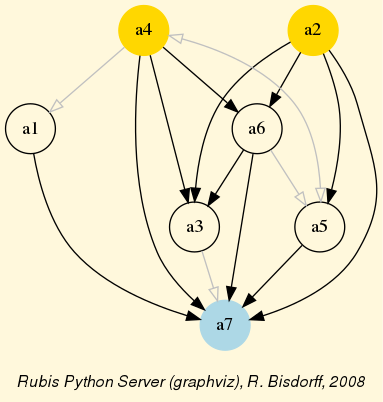
\includegraphics[width=7cm]{Figures/bestWorstOrientation.png}
\caption{The strict outranking digraph oriented by its initail and terminal prekernels. It becomes obvious here why alternative 'a1' is \emph{neither included nor excluded} from the initial prekernel. Same observation is applicable to alternative 'a3' which can \emph{neither be included nor excluded} from the terminal prekernel.}
%\label{fig:17.8}       % Give a unique label
\end{figure}
it may even happen, in case of more indeterminate outranking situations, that no alternative  is positively included or excluded from a weakly independent prekernel; the corresponding bipolar-valued membership characteristic vector being completely indeterminate (see for Listing \ref{list:x}).

To illustrate finally why sometimes we need to operate an epistemic disjunctive fusion of unequal stable low and high membership characteristics vectors (see Step 2.c.), let us consider, for instance, the following crisp 7-cycle graph.
\begin{lstlisting}
>>> g = CirculantDigraph(order=7,circulants=[-1,1])
>>> g			     
  *------- Digraph instance description ------*
   Instance class      : CirculantDigraph
   Instance name       : c7
   Digraph Order       : 7
   Digraph Size        : 14
   Valuation domain    : [-1.00;1.00]
   Determinateness (%) : 100.00
   Attributes          : ['name','order','circulants',
                          'actions','valuationdomain',
                          'relation','gamma','notGamma']
\end{lstlisting}		       

Digraph $c7$ is a symmetric crisp digraph showing, among others, the maximal independent set \{'2','5','7'\}, i.e. an initial as well as terminal kernel. We may compute the corresponding initial kernel characteristic vector.
\begin{lstlisting}
>>> g.computeKernelVector(['2','5','7'],\
...                       Initial=True,Comments=True)
 --> Initial kernel: {'2', '5', '7'}
 initial low vector  : [-1.0, -1.0, -1.0, -1.0, -1.0, -1.0, -1.0]
 initial high vector : [+1.0, +1.0, +1.0, +1.0, +1.0, +1.0, +1.0]
 1 st low vector     : [-1.0,  0.0, -1.0, -1.0,  0.0, -1.0,  0.0]
 1 st high vector    : [+1.0, +1.0, +1.0, +1.0, +1.0, +1.0, +1.0]
 2 nd low vector     : [-1.0,  0.0, -1.0, -1.0,  0.0, -1.0,  0.0]
 2 nd high vector    : [ 0.0, +1.0,  0.0,  0.0, +1.0,  0.0, +1.0]
 stable low vector   : [-1.0,  0.0, -1.0, -1.0,  0.0, -1.0,  0.0]
 stable high vector  : [ 0.0, +1.0,  0.0,  0.0, +1.0,  0.0, +1.0]
 Iterations          : 3
 low & high fusion   : [-1.0, +1.0, -1.0, -1.0, +1.0, -1.0, +1.0]
 Choice vector for initial prekernel: {'2', '5', '7'}
    '7': +1.00
    '5': +1.00
    '2': +1.00
    '6': -1.00
    '4': -1.00
    '3': -1.00
    '1': -1.00
\end{lstlisting}
Notice that the stable low vector characterises the \emph{negative membership} part, whereas, the stable high vector characterises the \emph{positive membership} part (see Lines 10-11 above).The bipolar epistemic fusion assembles eventually both stable parts into the correct prekernel characteristic vector (Line 13). 

The adjacency matrix of a symmetric digraph staying \emph{unchanged} by the transposition operator, the previous computations, when qualifying the same kernel as a terminal instance, will hence produce exactly the same result.

It is worthwhile noticing the essential computational role, the logical indeterminate value $0.0$ is playing in this double fixpoint algorithm. To implement such kind of algorithms without a logical \emph{neutral} term would be like implementing numerical algorithms without a possible usage of the number $0$. Infinitely many trivial impossibility theorems and dubious logical results come up. 
